\documentclass[10pt]{report}
%
\def\correction{0} % commenter cette ligne pour cacher les corrections.
%

\usepackage[a4paper]{geometry}
\usepackage{mathrsfs}
\usepackage{amssymb}
\usepackage{amsmath}
\usepackage{multicol}
\usepackage{graphicx}
\usepackage{subcaption}

\usepackage{enumitem}
\setlist[enumerate]{wide,labelindent=0cm,label=\textnormal{(\roman*)}}

\usepackage{tikz,pgfplots}
\pgfplotsset{compat=1.17}
\usepackage{caption}
\usepackage{float} % Required for the [H] float option
\usepackage{hyperref}

\DeclareMathOperator\atanh{atanh}

\newtheorem{exercice}{Exercice}

\usepackage{environ}

\newcommand{\K}{\mathbf{K}}
\newcommand{\R}{\mathbf{R}}
\newcommand{\N}{\mathbf{N}}
\newcommand{\Q}{\mathbf{Q}}
\newcommand{\C}{\mathbf{C}}
\newcommand{\Z}{\mathbf{Z}}
\newcommand{\ii}{\mathrm{i}}
\renewcommand{\leq}{\leqslant}
\renewcommand{\geq}{\geqslant}

\begin{document}

\noindent

\noindent
{\bf DTU Wind \& Energy System \hfill  COM section\\}
{\bf Emilien GOUFFAULT}

%% Figure on the upper right corner
\begin{figure}[H]
    \centering
    
\includegraphics[width=0.2\textwidth]{figures/dtuwindenergy_logo.jpeg}
\end{figure}


\begin{center}
{\bf Modeling of trajectories and impact velocities of droplets up-stream of a rain erosion test specimen or a turbine airfoil.}
\end{center}

\section*{Abstract}
\par Rain erosion is a major issue for wind turbine blades, particularly in offshore wind farms. The impact of raindrops on the blades can cause significant damage, leading to reduced efficiency or halted activity and increased maintenance costs. This erosion is due to the impact speed of droplets on the blade, as demonstrated by Bech in 2022 \cite{Bech2022}. In this report, we present a model to predict the trajectories and impact velocities of droplets on turbine airfoils. The model takes into account droplet deformation and the air velocity around the blade. We aim to provide a better understanding of droplet behavior and its impact on turbine blades and on Rain Erosion Tests (RET). The model is based on the work of Sor and Garcia-Magariño \cite{Sor2016} and Barfknecht \cite{Barfknecht2024}.
\par It appears that the three main parameters governing droplet behavior are the droplet diameter, the airfoil geometry, and a parameter, \( n \), linking the air velocity to the distance between the droplet and the blade. The droplet diameter is the most important parameter, as it significantly affects droplet deformation, fall speed, and impact velocity. The airfoil geometry also plays a crucial role, as it influences the air velocity around the blade and the droplet trajectory. Finally, the parameter \( n \) is important for calculating the air velocity, as it determines how quickly the air velocity decreases with distance from the blade. We show that this model can be used to predict the impact velocities of droplets on turbine blades and to optimize RET conditions.

\section*{Tutors and contacts}
I am tutored by three researchers from the DTU Wind \& Energy Systems, who are experts in the field of rain erosion and turbine aerodynamics. They are helping me to understand the physical phenomena governing droplet behavior and to apply the model to real turbines. They are also providing me with meteorology data to estimate the lifetime expectancy of turbine blades in the context of rain erosion. Jakob is the one really monitoring my internship, while Mac and Ásta are helping me with the model and the meteorology data.
\begin{itemize}
    \item Jakob Ilsted Bech, DTU Wind \& Energy Systems, Composites Manufacturing and Testing, \url{jakb@dtu.dk} \
    \item Mac Gaunaa, Department of Wind and Energy Systems, Wind Turbine Design Division, \url{macg@dtu.dk}\
    \item Ásta Hannesdóttir, Department of Wind and Energy Systems, Meteorology and Remote Sensing, \url{astah@dtu.dk}
\end{itemize}

\newpage

\section*{Introduction}

\section*{Model and simulation}

\subsection*{Presentation}
\par The droplets are generated by a droplet generator head, which is a device that generates droplets of a given diameter $d$ and velocity. The droplets are then falling down in the air, and we want to model their trajectory and impact velocity on an airfoil, approaching at a certain speed.
\par For this first part, we will track $x,y$ the coordinates of the droplet in space, $a$ and $b$ the largest and smallest semiaxis of the oblate spheroid, and $t$ the time. The droplet is assumed to be an oblate spheroid, which is a sphere that has been deformed by the air flow. The droplet is initially a sphere of radius $R$, and its deformation is ruled by three forces: the viscous force, the flow pressure force and the surface tension force.
\begin{figure}[H]
    \centering
    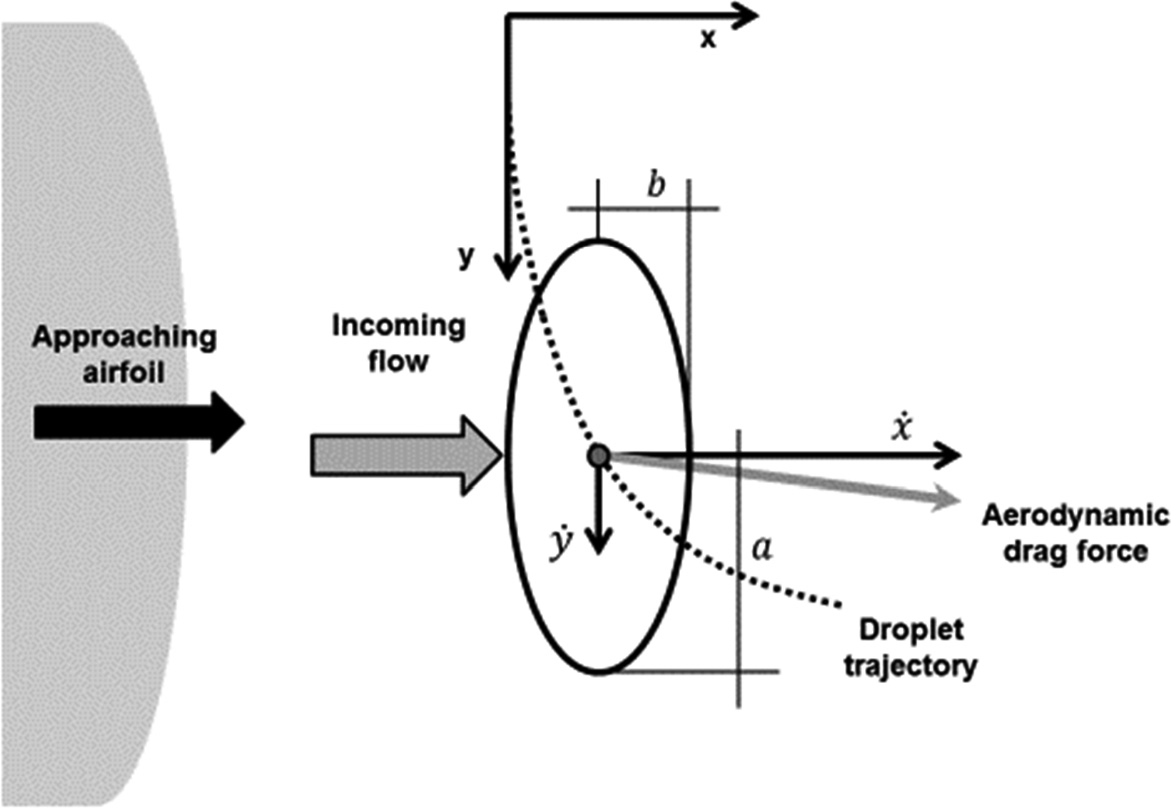
\includegraphics[width=0.8\textwidth]{figures/scheme_model.png}
    \caption{Scheme of the model}
\end{figure}

\subsection*{Model description}

    \par The behaviour of the droplets is separated into two parts: the trajectory and the droplet deformation. The trajectory is ruled by various forces : 
\begin{itemize}
    \item the drag force, which is proportional to the square of the velocity and acts in the opposite direction of the droplet motion,
    \item the gravitational force, which acts in the direction of the droplet motion,
    \item the pressure gradient force, which acts in the direction of the droplet motion and is proportional to the droplet diameter and the air density,
    \item the virtual mass force, which acts in the direction of the droplet motion and is proportional to the droplet diameter and the air density,
\end{itemize}
\par Regarding the fact that the volumic mass of water, $\rho$, is approximately 1000 times greater than $\rho_{air}$, the pressure gradient force and the virtual mass force are negligible compared to the drag force and the gravitational force. 

\vspace{5mm}
Furthermore, the droplet deformation is assumed to be an oblate spheroid, which is initially a sphere of radius $R$. Its deformation is ruled by three forces:
\begin{itemize}
    \item the viscous force, which acts in the opposite direction of the droplet motion and is proportional to the square of the velocity,
    \item the flow pressure force, which tends to deform the droplet,
    \item the surface tension force, which counteracts with the flow pressure force,
\end{itemize}

Thus, we have the following \textbf{equation of motion for the droplet}:

\begin{align}
    m\frac{d^2x}{dt^2} &=  F_x \\
    m\frac{d^2y}{dt^2} &= -F_y + mg \\
    \frac{3m}{16}\frac{d^2a}{dt^2} &= F_v + F_p + F_s 
\end{align}

Where:
\begin{itemize}
    \item $m = \frac{4}{3}\pi R^3 \rho$ is the droplet mass
    \item $F_x$, $F_y$ is the drag force in the $x$ and $y$ direction
    \item $F_v$ is the viscous force
    \item $F_p$ is the flow pressure force
    \item $F_s$ is the surface tension force
\end{itemize}\par 

One important variable to calculate the drag force is the slip velocity, which is the difference between the droplet velocity and the air velocity. The slip velocity is given by:
\begin{align}
    v_{x} &= v_{air} - \frac{dx}{dt}, \\
    v_{y} &= \frac{dy}{dt}.
\end{align}

\par We assume that $v_{x}  \gg  v_{y}$, which means that the droplet is moving much faster in the $y$ direction than in the $x$ direction. This assumption is valid for small droplets, which are moving at low velocities.

\par We used Barfknecht's model \cite{Barfknecht2024} to describe the air velocity. The air velocity, in the droplet referential, is given by:

\begin{align}
    v_{air} &= v_{b} \times \frac{1}{\left(1+\frac{\Delta x}{R_c(\alpha)}\right)^{n}}
\end{align}

where $v_{b}$ is the velocity of the blade, $\Delta x$ is the distance between the droplet and the blade, $R_c(\alpha)$ is the radius of curvature of the blade at angle $\alpha$, and $n$ is a constant that depends on the blade profile.

Therefore, the droplet instantaneous frontal area is given by $A = \pi a^2$. Thus, we can write the \textbf{drag force in the $x$ direction} as:
\begin{align}
    F_x &= \frac{1}{2} \rho_{air} v_{x}^2 \pi a^2 C_D
\end{align}
where $C_D$ is the \textbf{drag coefficient}, composed of two parts: a static one (which is a combination of the drag coefficient of a sphere and the drag coefficient of an oblate spheroid) and a dynamic one :
\begin{align}
    C_D &= C_{stat} + C_{dyn} \\
    C_{stat} &= C_{D,sphere}^{\frac{b}{a}} C_{D,disk}^{1-\frac{b}{a}} \\
    C_{dyn} &= k \frac{b}{v_{x}^2}\frac{dv_{x}}{dt}
\end{align}
here $C_{D,sphere}$ and $C_{D,disk}$ are the drag coefficients of a sphere, depending on the Reynolds number, and a disk, considered constant for the Reynolds number of the droplet. $k$ is a calibration constant in order to fit the experimental data.

\par We can rewrite $C_{dyn}$ as:
\begin{align}
    C_{dyn} &= k \frac{b}{v_{x}^2}\left(\frac{d}{dt}\left(v_{air} - \frac{dx}{dt}\right)\right) \\
            &= k \frac{b}{v_{x}^2}\left(\frac{nv_{b}\left(v_{b}-\frac{dx}{dt}\right)}{R_c(\alpha)\left(1+\frac{\Delta x}{R_c(\alpha)}\right)^{n+1}}-\frac{d^2x}{dt^2}\right) \\
            &= C_{dyn,1} - C_{dyn,2} 
\end{align}

thus we can write the equation $(1)$ as:
\begin{align}
    \left(m + \frac{1}{2}k\rho_{air}\pi b a^2\right)\frac{d^2x}{dt^2} &= \frac{1}{2} \rho_{air} v_{x}^2 \pi a^2 \left(C_{stat} + C_{dyn,1}\right)
\end{align}
where we have added the term $\frac{1}{2}k\rho_{air}\pi b a^2$ to the mass of the droplet, which is the mass of the air that is dragged by the droplet. This term is negligible compared to the mass of the droplet, but it is important for the calculation of the drag force.

\par Similarly, we can write the \textbf{drag force in the $y$ direction}:
\begin{align}
    F_y &= \frac{1}{2} \rho_{air} v_{y} v_{x} \pi a^2 C_D
\end{align}

\par The \textbf{viscous force} is given by:
\begin{align}
    F_v &= -\frac{64}{9} \mu \pi R^3 \frac{1}{a^2} \frac{da}{dt}
\end{align}
where $\mu$ is the air dynamic viscosity. This force is described as negligible compared to the two following according to Sor and Garcia-Magariño \cite{Sor2016}.

\par The \textbf{flow pressure force} is given by:
\begin{align}
    F_p &= \frac{1}{2} \rho_{air} v_{x}^2 \pi R^2 C_P
\end{align}
where $C_P$ is the pressure coefficient, that has been calibrated by Sor and Garcia-Magariño \cite{Sor2016} in order to fit the experimental data. We take $C_P =0.93$. Ibrahim and al. \cite{Ibrahim2014} explains that this force is propotional to $R$ and not to $a > R$ due to the decreasing pressure during the droplet falldown.

\par In order to define the surface tension force we first need to define the surface area of an oblate spheroid $A_d$. This is given by:
\begin{align}
    A_d &= 2 \pi a^2 + 2 \pi \frac{R^6}{a^4}\frac{\atanh{\left(\sqrt{1-\left(\frac{b}{a}\right)^2}\right)}}{\sqrt{1-\left(\frac{b}{a}\right)^2}}
\end{align}

Finally, the \textbf{surface tension force} is given by:
\begin{align}
    F_s &= -\frac{4}{3}\sigma\frac{dA_d}{da}
\end{align}
which is, if we note the excentricity $\epsilon := \sqrt{1-\left(\frac{b}{a}\right)^2}$:

\begin{align}
    F_s &= -\frac{4}{3}\sigma\left(4\pi a + 2 \pi \frac{R^6}{a^5 \epsilon}\left(\frac{3}{\epsilon} - \atanh(\epsilon)\left( 1  + \frac{3}{\epsilon^2}\right)\right)\right)
\end{align}
\vspace{5mm}

\par In theory, our model allows the droplets to deform and to grow infinitely, but in practice the droplet will eventually break up due to the air velocity and the surface tension force. In this study, we assume that the droplet will break up when $a$ is greater than a certain threshold $a_{max}$ according to Barfknecht (2024) \cite{Barfknecht2024}, which is the maximum radius of the droplet. This threshold is a function of the Weber number  $\text{We}_{\infty} = \frac{\rho_{\text{air}}V_{\infty}^2 d}{\sigma_{\text{water}}} $ and is given by:
\begin{align}
    \frac{a_{\text{max}}}{R} = \min(2.2,3.4966 \text{We}_{\infty}^{-0.1391})
\end{align}
This value was obtained by Barfknecht (2024) \cite{Barfknecht2024} from experimental data and a regression. If the droplet radius exceeds this threshold, we assume that the droplet will have reached its maximum size and $a$ will be set to $a_{max}$ for the rest of the simulation. Note that here, $R = \frac{d}{2}$ is the initial radius of the droplet, $V_{\infty}$ is the blade velocity, and $\sigma_{\text{water}}$ is the surface tension of water.
\par After many tests, we realized that for the parameters that interest us, $a$ reached $a_max$ only for large droplets and at the very end of the simulation (right before hiting the blade). Thus, we can assume that the droplet will not break up during its fall, and we can use the model to predict the impact velocity of the droplet on the blade.
\vspace{5mm}
\par Furthermore, in order to calculate the droplet fall speed, we use Foote and Du Toit's \cite{foote1969terminal} model (1969). Their model is based on an interpolation of the droplet diameter and the fall speed, which is given by:
\begin{align}
    V_f(d) &= \sum_{i=1}^{n} A_i d^i
\end{align}

where $A_i$ are the coefficients of the interpolation, which are given by Foote and Du Toit \cite{foote1969terminal} for different droplet diameters. The fall speed is then used to calculate the initial velocity of the droplet.

\subsection*{Model validation}
\par In order to validate our model, we used data from Vargas (2011) \cite{Vargas2010}. In their experiment, they use a setup identical to our model setup, generating droplets of known diameter and measuring their trajectories and impact velocities under controlled conditions. We simulated the same experimental conditions using our model, setting the droplet diameter, initial velocity, and air properties to match those reported by Vargas, which was droplets with a $0.98mm$ diameter, and we used $R_c(\alpha) = 7.1 \mathrm{cm}$ and $n=1.3$.
\vspace{5mm}
\par Figure~\ref{fig:vargas_comparison} shows the comparison between the experimental data from Vargas and the results predicted by our model for the droplet trajectory and impact velocity. The x-axis represents the distance between the airfoil and the droplet and the y-axis shows the difference of velocity (i.e. the speed reduction). The line is the result of our model, and the dots are the data measured by Vargas. The agreement between the two is very good, we can see a larger error for the highest speeds which can be due to more irregularity in the air velocity.
\begin{figure}[H]
    \centering
    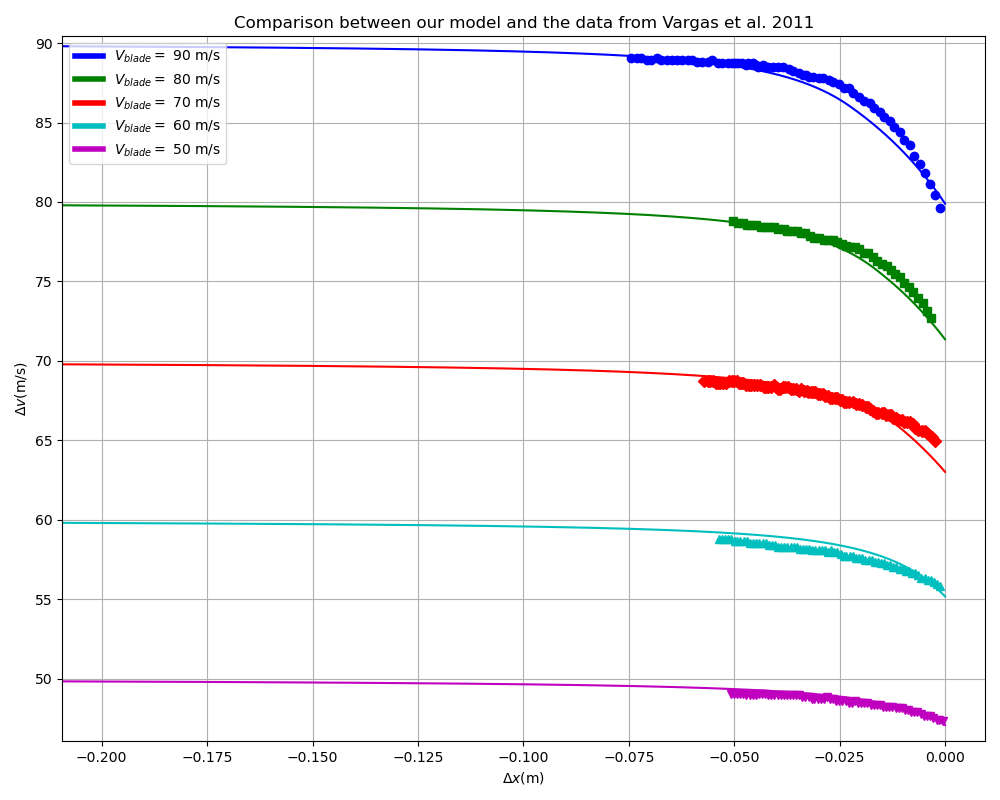
\includegraphics[width=1\textwidth]{figures/comp_vargas.png}
    \caption{Comparison between Vargas (2011) experimental data and model predictions for droplet trajectory and impact velocity.}
    \label{fig:vargas_comparison}
\end{figure}

\par These results confirm that our model accurately captures the main physical phenomena governing droplet motion and deformation in the context of rain erosion testing. This validation gives confidence in using the model for further simulations and for optimizing RET conditions.
\vspace{5mm}
\par Furthermore we also verified the droplets fall speed to validate Foote and Du Toit's model. We used the same experimental conditions as in Vargas (2011) \cite{Vargas2010} and compared the fall speed predicted by our model with the fall speed measured by Vargas. The results are shown in Figure~\ref{fig:fall_speed_validation}. The x-axis represents the droplet diameter and the y-axis shows the fall speed. The line is the result of our model, and the dots are the data measured by Vargas. The agreement between the two is very good, which confirms that our model accurately captures the droplet fall speed.
\begin{figure}[H]
    \centering
    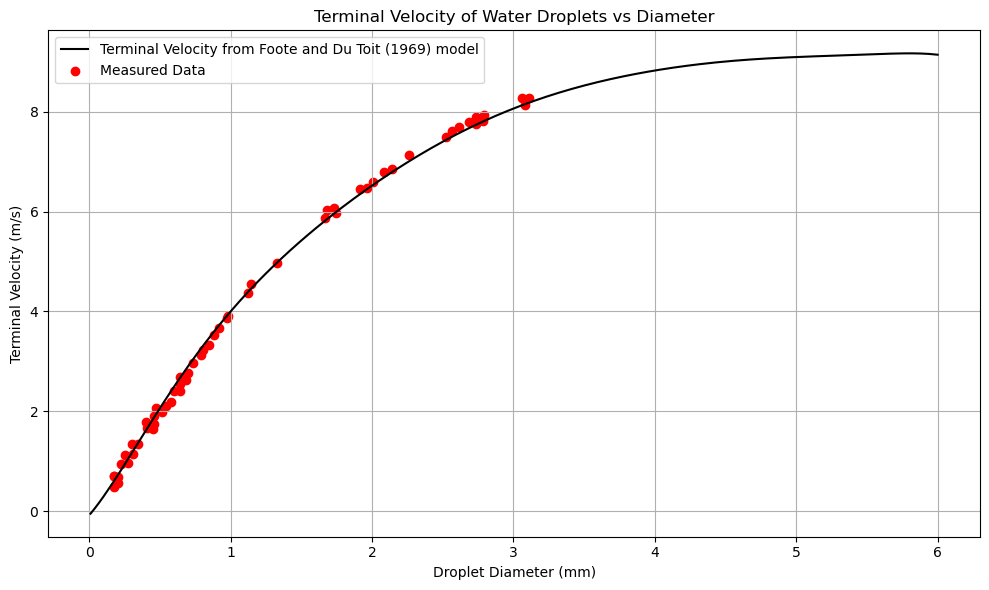
\includegraphics[width=0.8\textwidth]{figures/fall_speed_validation.png}
    \caption{Comparison between Vargas (2011) experimental data and model predictions for droplet fall speed.}
    \label{fig:fall_speed_validation}
\end{figure}

\section*{Impact on the rain erosion tester (RET)}

\par The objective of this model is to enhance our understanding of droplet behavior in the context of Rain Erosion Testing (RET). Historically, the impact velocity used in RET experiments has been approximated using the formula \( V = \Omega R \), where \( V \) represents the rotor speed at a distance \( R \) from the rotor center, rotating at an angular speed $\Omega$. This simplification assumes that droplets maintain a velocity consistent with the rotor speed at the point of impact, neglecting potential variations due to aerodynamic drag, turbulence, or other environmental factors.
\par However, this assumption may not fully capture the complexities of real-world scenarios, where droplets could be subjected to deceleration due to various forces acting upon them. Consequently, a key focus of this study is to investigate and quantify the extent to which droplets are decelerated as they approach the rotor blades. Understanding this deceleration is crucial for accurately predicting the erosion patterns and rates experienced by turbine blades in operational conditions.
\par By refining our knowledge of droplet dynamics, this model aims to provide a more precise framework for evaluating and mitigating rain erosion effects on turbine blades. This, in turn, will contribute to the development of more durable and efficient turbine designs, ultimately enhancing their performance and longevity in diverse environmental conditions.

\subsection*{Impact speed and lifetime expectancy}

The analysis presented in Figure~\ref{fig:rain_tester} illustrates the deceleration experienced by droplets of varying diameters as they approach the specimen in a Rain Erosion Test (RET). The foundational data for this analysis were derived from the work of Bech \cite{Bech2022}. In this figure, the x-axis denotes the expected lifetime of a blade until the first crack appears, while the y-axis represents the impact speed, which can either be the blade speed or the corrected speed accounting for droplet deceleration.

For our simulation, we utilized a radius of curvature of the blade defined as \( R_c(\alpha) = 4.455 \, \text{mm} \) and a parameter \( n = 1.1 \). These parameters were chosen to closely mimic real-world conditions and to provide insights into how different droplet sizes behave under similar aerodynamic forces. By examining the deceleration patterns, we aim to better understand the dynamics of droplet impact and its implications for blade erosion and longevity. This understanding is crucial for developing more accurate predictive models and for enhancing the design and material selection of turbine blades to withstand erosive forces in operational environments.

\begin{figure}[H]
    \centering
    \begin{subfigure}[b]{0.7\textwidth}
        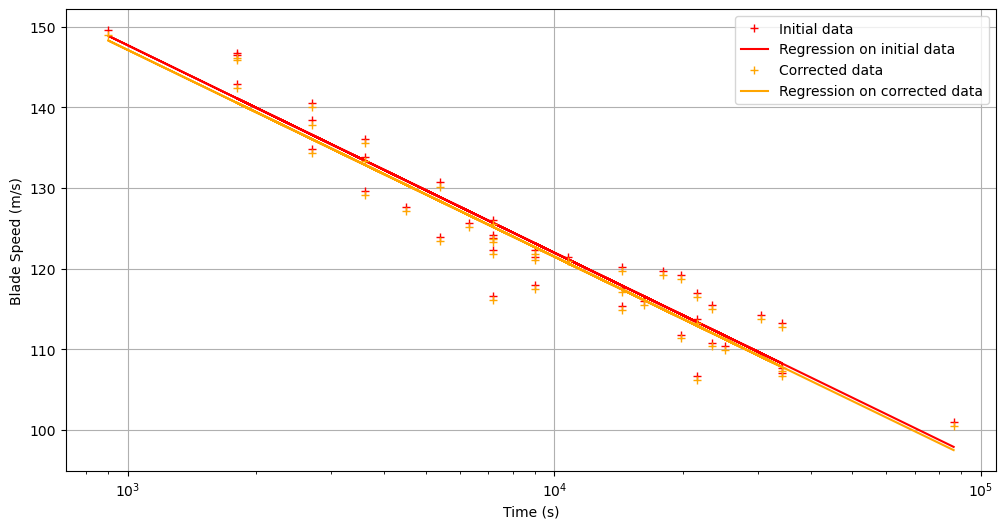
\includegraphics[width=\textwidth]{figures/ret_analysis_190.png}
        \caption{Speed correction for $d = 1.90 \mathrm{mm}$}
    \end{subfigure}
    \hfill
    \begin{subfigure}[b]{0.7\textwidth}
        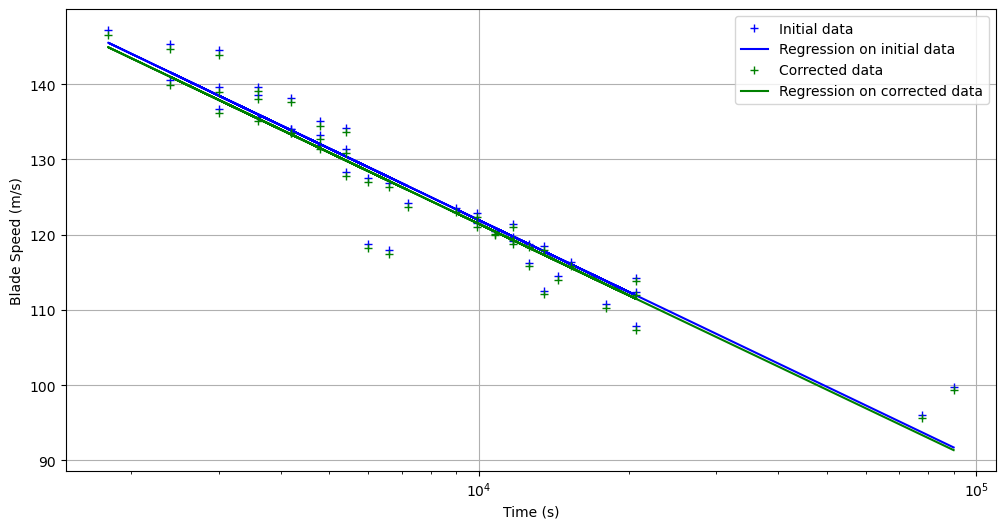
\includegraphics[width=\textwidth]{figures/ret_analysis_238.png}
        \caption{Speed correction for $d = 2.38 \mathrm{mm}$}
    \end{subfigure}
    \caption{RET speed correction}
    \label{fig:rain_tester}
\end{figure}

\par The results obtained demonstrate that the actual droplet impact velocity is very close to the blade velocity. Indeed, the effect highlighted in the first part of the study proves to be negligible in this context, as the blades are too thin to significantly influence droplet behavior. The corrected velocity does not differ by more than \(0.5 \, \text{m/s}\), which is an important first result. We can now assert that the work conducted with the Rain Erosion Test (RET) takes into account the correct impact velocity.
\par This validation of the RET's experimental conditions is crucial, as it confirms the reliability of the studies conducted to date. The research has enabled a thorough understanding of the mechanisms of rain erosion under controlled conditions, providing a solid foundation for further investigations.
\par The major challenge now lies in translating these experimental results to real turbines. It is essential to develop methods that allow these findings to be applied in operational conditions, in order to optimize the durability and performance of turbines against rain erosion. Future research will need to focus on adapting the parameters identified in the laboratory to the constraints and variations of real environments, thus ensuring an effective transition from theory to practice.



\section*{Translation to real turbines}

We can now utilize this model to predict the impact velocities of droplets on actual turbine blades. The subsequent step involves applying this model to real turbine blades, considering the blade geometry and the air velocity surrounding the blade.

\subsection*{Comparison of two turbines}

In this study, we compare two turbines with distinct blade profiles: the NREL 5MW turbine and the IEA 15MW turbine. The NREL 5MW turbine features a blade length of \(63 \, \text{m}\) and a maximum chord length of \(4.2 \, \text{m}\), whereas the IEA 15MW turbine has a blade length of \(107 \, \text{m}\) and a maximum chord length of \(6.5 \, \text{m}\). We maintain the same droplet diameter and air velocity as in the previous section and calculate the impact velocities on both turbines.

Figure~\ref{fig:comparison_turbines} illustrates the two primary parameters influencing the impact velocity: the curvature of the blade \(R_c(\alpha)\) and the parameter \(n\), which characterizes the air velocity around the blade. The x-axis represents the position on the blade, with \(r/R = 1\) at the tip of the blade.

\begin{figure}[H]
    \centering
    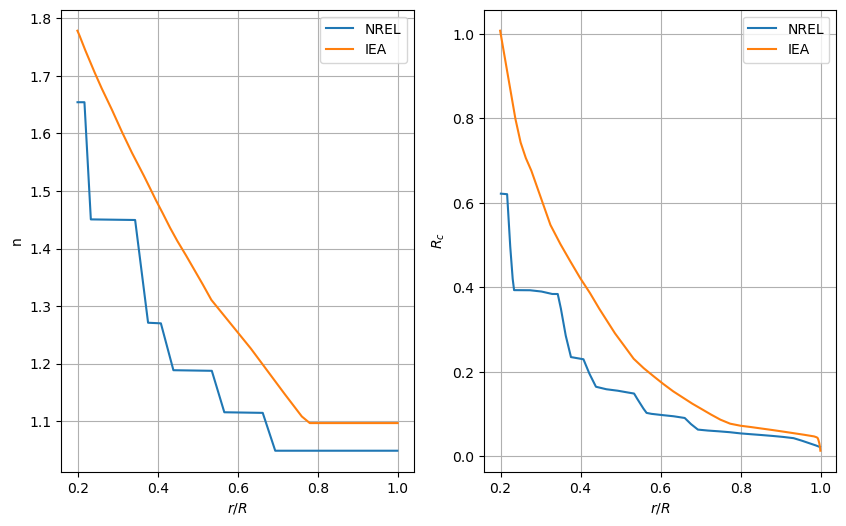
\includegraphics[width=0.7\textwidth]{figures/n_rc_comp.png}
    \caption{Comparison of blade geometry on NREL 5MW and IEA 15MW turbines.}
    \label{fig:comparison_turbines}
\end{figure}

We have slightly modified the model to account for the blade profile and the verticality of the air velocity. This modification includes the angle of the blade during impact, which is the angle between the blade and the horizontal plane, as depicted in Figure~\ref{fig:scheme_theta}.

\begin{figure}[H]
    \centering
    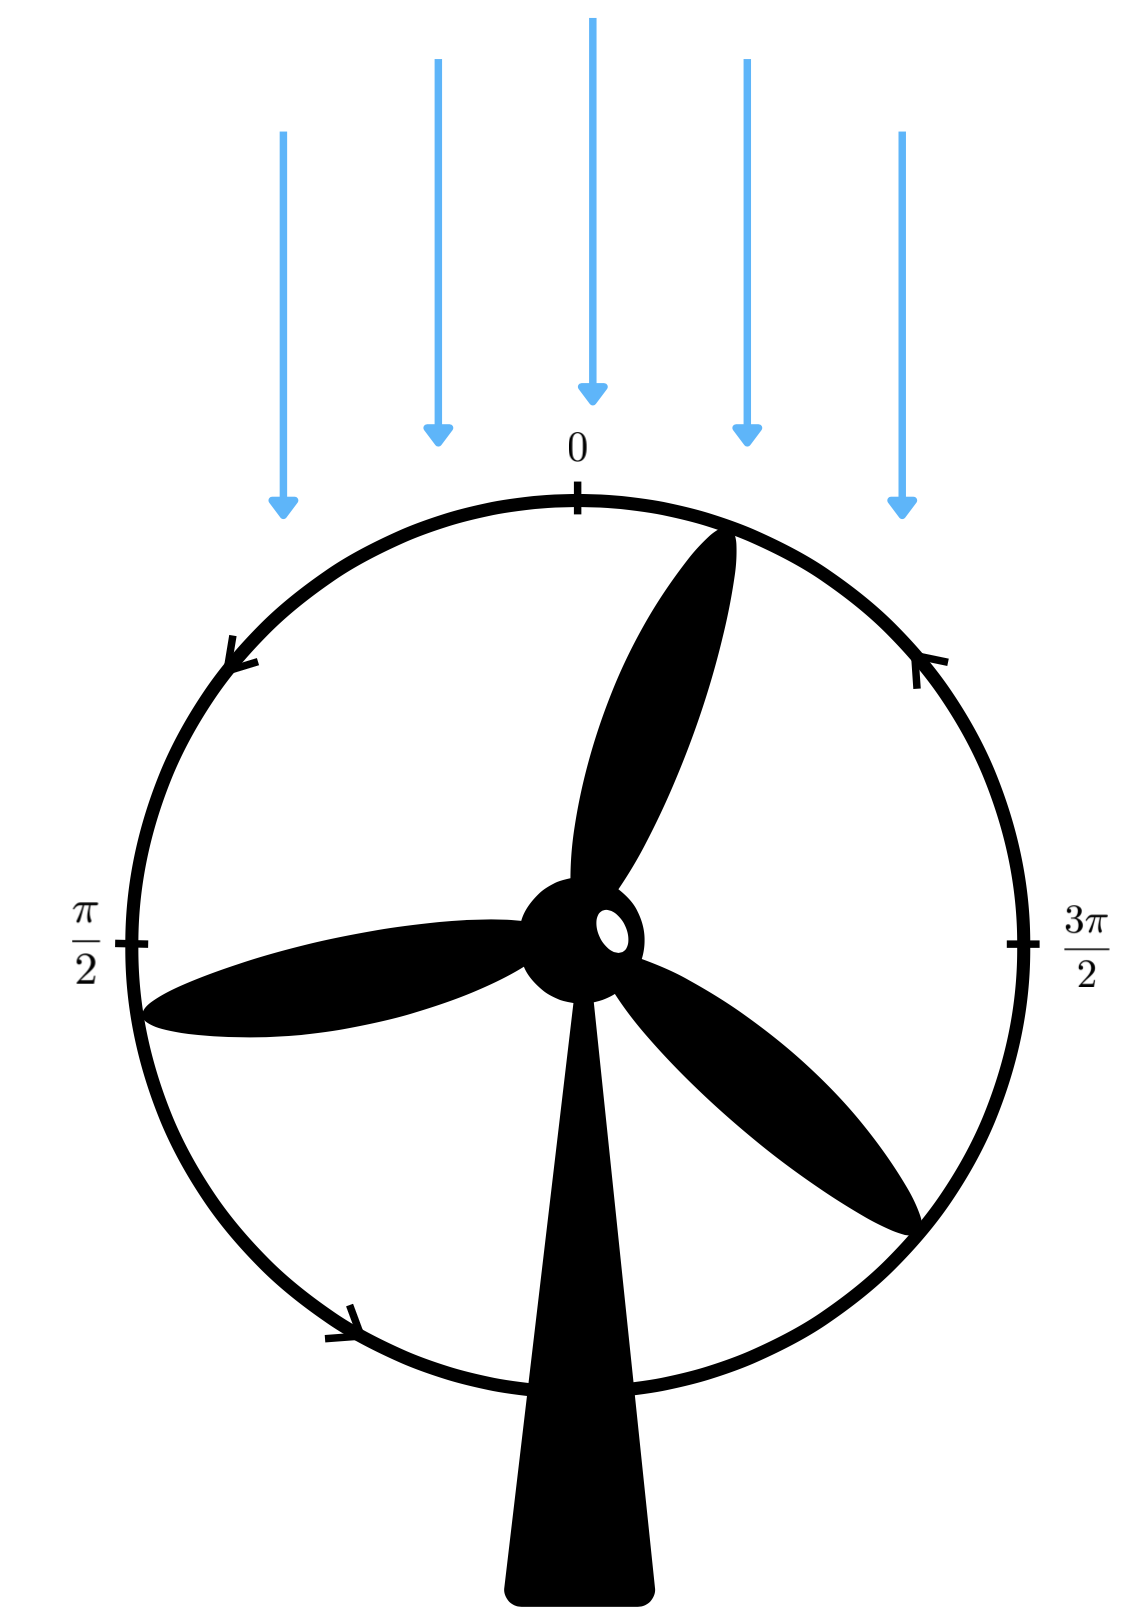
\includegraphics[width=0.5\textwidth]{figures/scheme_theta.png}
    \caption{Scheme of the model.}
    \label{fig:scheme_theta}
\end{figure}

Figure~\ref{fig:impact_velocity} shows the impact velocity of droplets on the two turbines, depending on the angle of impact, for a tip speed of \(95 \, \text{m/s}\) for the IEA 15MW turbine, and of \(80 \, \text{m/s}\) for the NREL 5MW turbine. These tip speeds correspond to the maximum speeds of the turbines according to their specifications \cite{NREL2009} \cite{IEA2020}.

The dotted line represents the impact velocity of droplets if we were not to consider the speed reduction studied in this paper. The solid line represents the impact velocity of droplets when considering the speed reduction. The impact velocity is significantly lower when accounting for the speed reduction, especially for larger droplets. This result confirms the importance of considering droplet deceleration in predicting impact velocities on turbine blades.
\begin{figure}[H]
    \centering
    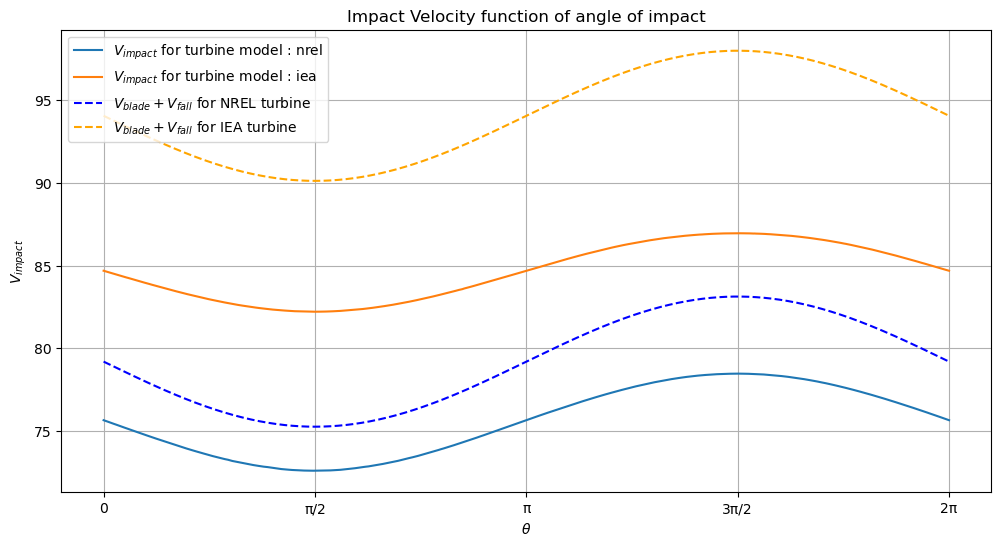
\includegraphics[width=0.8\textwidth]{figures/turbine_comp_angle.png}
    \caption{Impact velocity on NREL 5MW and IEA 15MW turbines at different angles of impact.}
    \label{fig:impact_velocity}
\end{figure}

Additionally, we conducted a comparison between the two turbines at a fixed angle of blade of $\frac{3 \pi}{2}$ in order to have the maximum impact speed. This time, the x-axis represents the distance to the center of the blade and the y-axis shows the impact velocity of droplets on the blade. The results are presented in Figure~\ref{fig:impact_velocity_comp} for a tip speed of \(80 \, \text{m/s}\) for the NREL 5MW turbine and \(95 \, \text{m/s}\) for the IEA 15MW turbine as explained before.

\begin{figure}[H]
    \centering
    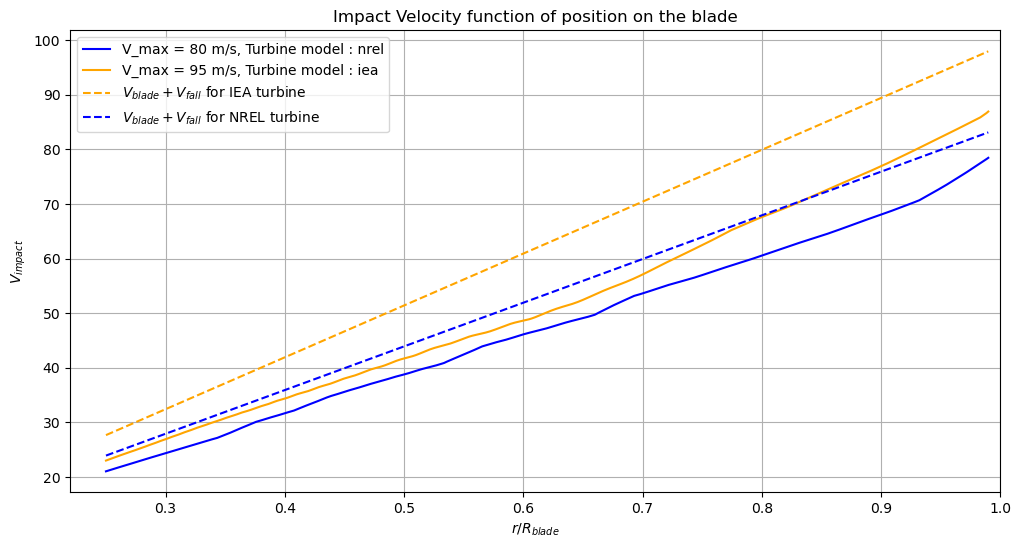
\includegraphics[width=0.8\textwidth]{figures/turbine_comp.png}
    \caption{Impact velocity of droplets on NREL 5MW and IEA 15MW turbines along the blade.}
    \label{fig:impact_velocity_comp}
\end{figure}

As we can see, the speed reduction is significantly greater for the IEA 15MW turbine than for the NREL 5MW turbine. This is due to the larger blade length and chord length of the IEA 15MW turbine, which results in a greater distance between the droplet and the blade, leading to a greater speed reduction. This result confirms that the blade geometry plays a crucial role in droplet behavior and impact velocities.

Furthermore, we observe that even if the IEA 15MW turbine has a $15 \mathrm{m/s}$ higher tip speed, the impact velocity of droplets on the blade is only $9 \mathrm{m/s}$ higher. Thus, the impact of building larger turbines is not necessarily detrimental to the impact velocity of droplets on the blade, as long as the blade geometry is optimized to increase droplet deceleration.
\subsection*{Lifetime Expectancy of the Blades}
We now conduct a study of the lifetime expectancy of the blades based on the impact velocities calculated in the previous section. The lifetime expectancy is defined as the time it takes for a blade to reach a certain level of damage due to rain erosion. This level of damage is defined as the point at which the blade is no longer able to withstand the impact of droplets and fails.
\subsubsection*{Model Description}
In order to define properly the lifetime expectancy of the blades, we need to define impingement, which is the amount of water that the blade will encounter during its lifetime. Bech (2022) \cite{Bech2022} shows, with a power law function, that the impingement can be expressed as a funciton of the impact velocity :
\begin{align}
    N(v,d) = c(d)\times v^{-m(d)}
\end{align}
Lifetime calculations are then done, using Palmgren-Miner’s rule, as suggested by Slot (2015) \cite{SLOT2015837}. The linear summation of damage increments using the Palmgren-Miner rule results in the accumulated damage sum (D) given by :
\begin{align}
    D = \sum_{i=1}^{n} \int_{0}^{2\pi} \frac{n_i(v,d,\theta)}{N_i(v,d)} d\theta
\end{align}
where every step of the summation represents the damage caused during a period of time $dt$ by the impact of droplets with a velocity $v$ and diameter $d$, for blades spinning between $0$ and $2\pi$. The damage is calculated using the amount of impinged water during bin $i$ : $n_i(v,d,\theta)$ and the impingement $N_i(v,d)$, which is the amount of impinged water that can be tolerated before the blade fails.

We can express the amount of impinged water during a period of time $dt$ as:
\begin{align}
    n_i(v,d,\theta) = \frac{I}{v_{fall}(I)} (v_{blade} - \sin(\theta)\times v_{fall}) dt
\end{align} 
where $I$ is the rain intensity, $v_{fall}(I)$ is the fall speed of the droplets, $v_{blade}$ is the blade speed, and $\theta$ is the angle of the blade (Figure~\ref{fig:scheme_theta}). The term $(v_{blade} - \sin(\theta)\times v_{fall})$ represents the relative velocity between the droplet and the blade, which is the velocity at which the droplet impacts the blade without speed reduction. The term $\frac{I}{v_{fall}(I)}$ is the amount of water that the droplet will encounter during its fall, which is proportional to the rain intensity and inversely proportional to the fall speed of the droplet.

Finally, when $D=1$, the blade is considered to have failed and we obtain the lifetime expectancy of the blade.

\subsubsection*{Simulation and Results}
We conducted a simulation to estimate the lifetime expectancy of the blades based on the impact velocities calculated in the previous section. We used the same methodology as in the previous section, but this time we used Hannesdóttir's model and code \cite{hannesdottir2024} and data from era5.

\section*{Conclusion}
\bibliographystyle{plain}
\bibliography{references}

\end{document}